%%-------------------------------------------------------------------------------------- Início
\begin{frame}[allowframebreaks, t, fragile]{Ação: Create}
  \begin{figure}[h!]
		\centering
		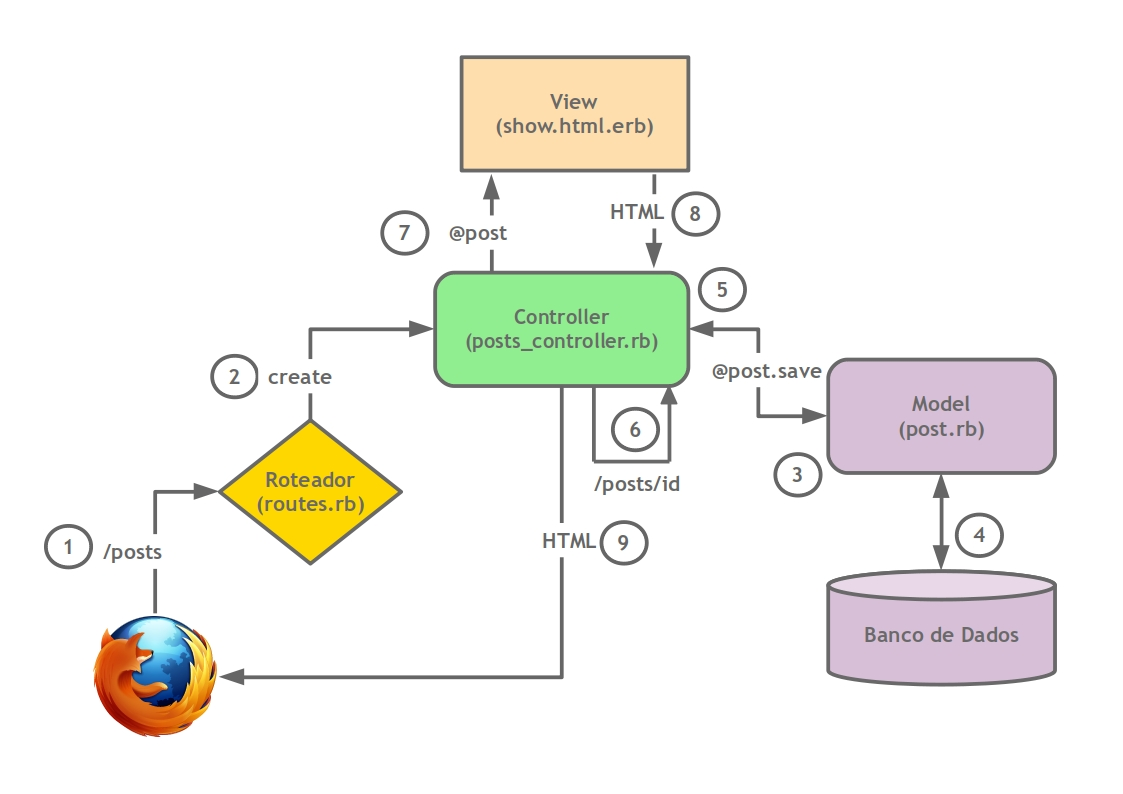
\includegraphics[width=0.75\textwidth]{imagens/mvc-action-create.jpg}
	\end{figure}
	\framebreak
  \begin{itemize}
		\item Um novo objeto \alert{@post} da classe \alert{Post} é criado com os parâmetros que foram passados pelo 
			formulário \alert{new}
		\item Tenta \alert{salvar} o objeto \alert{@post} no \alert{banco de dados}
%		\item Se sucesso, redireciona para o template \alert{show}
%		\item Se insucesso, renderiza o template \alert{new} novamente
		\begin{lstlisting}[style=RubyInputStyle, caption=controllers/posts\_controller.rb]
class PostsController < ApplicationController
  def new
      @post = Post.new
  end

  def create 
      @post = Post.new(post_params)
      
      @post.save
      redirect_to @post
  end

private 
  def post_params 
    params.require(:post).permit(:title, :body)
  end
end          
		\end{lstlisting}		
		\begin{itemize}
			\item a linha 15 implementa \alert{strong parameters} para aumentar a segurança da aplicação
    \end{itemize}
    \item Como a ação {\bf Show} ainda não foi implementada, ocorrerá uma erro quando
    o botão {\bf Submit} for pressionado.
	\end{itemize}	
\end{frame}